\part{Analytic Number Theory}

\chapter{Prime Numbers}

\section{Fundamental Definitions}

\begin{definition}[Prime number]
  An integer $p > 1$ is \emph{prime} if its only positive divisors are $1$ and $p$. The set of all primes is denoted $\mathbb{P} = \{2, 3, 5, 7, 11, 13, \ldots\}$.
\end{definition}

\begin{theorem}[Euclid's theorem]
  There are infinitely many prime numbers.
\end{theorem}

\begin{proof}
  Suppose there are only finitely many primes $p_1, p_2, \ldots, p_n$. Consider $N = p_1 p_2 \cdots p_n + 1$. Then $N > 1$, so $N$ has a prime divisor $p$. But $p$ cannot be any $p_i$, since $N \equiv 1 \pmod{p_i}$. This contradicts the assumption that $p_1, \ldots, p_n$ are all the primes.
\end{proof}

\begin{theorem}[Fundamental theorem of arithmetic]
  Every integer $n > 1$ can be written uniquely (up to order) as a product of primes:
  \begin{equation}
    n = p_1^{a_1} p_2^{a_2} \cdots p_k^{a_k},
  \end{equation}
  where $p_1 < p_2 < \cdots < p_k$ are primes and $a_i \geq 1$.
\end{theorem}

\begin{definition}[Prime counting function]
  The \emph{prime counting function} $\pi : \mathbb{R} \to \mathbb{Z}_{\geq 0}$ is defined by
  \begin{equation}
    \pi(x) = \#\{p \leq x : p \text{ is prime}\} = \sum_{p \leq x} 1.
  \end{equation}
\end{definition}

The central question of analytic number theory is: \emph{How does $\pi(x)$ grow as $x \to \infty$?}

\section{Arithmetic Functions}

\begin{definition}[Arithmetic function]
  An \emph{arithmetic function} is a function $f : \mathbb{Z}_{>0} \to \mathbb{C}$.
\end{definition}

\begin{definition}[Multiplicative functions]
  An arithmetic function $f$ is:
  \begin{itemize}
    \item \emph{Multiplicative} if $f(mn) = f(m)f(n)$ whenever $\gcd(m,n) = 1$.
    \item \emph{Completely multiplicative} if $f(mn) = f(m)f(n)$ for all $m, n$.
  \end{itemize}
\end{definition}

\begin{definition}[Dirichlet convolution]
  The \emph{Dirichlet convolution} of arithmetic functions $f$ and $g$ is
  \begin{equation}
    (f * g)(n) = \sum_{d \mid n} f(d) g\left(\frac{n}{d}\right) = \sum_{ab = n} f(a) g(b).
  \end{equation}
\end{definition}

\begin{proposition}
  Dirichlet convolution is associative and commutative. The identity element is
  \begin{equation}
    \varepsilon(n) = \begin{cases} 1 & \text{if } n = 1, \\ 0 & \text{if } n > 1. \end{cases}
  \end{equation}
\end{proposition}

\subsection{The M\"obius Function}

\begin{definition}[M\"obius function]
  The \emph{M\"obius function} $\mu : \mathbb{Z}_{>0} \to \{-1, 0, 1\}$ is defined by
  \begin{equation}
    \mu(n) = \begin{cases}
      1      & \text{if } n = 1,                                            \\
      (-1)^k & \text{if } n = p_1 p_2 \cdots p_k \text{ (distinct primes)}, \\
      0      & \text{if } p^2 \mid n \text{ for some prime } p.
    \end{cases}
  \end{equation}
\end{definition}

\begin{proposition}
  For all $n \geq 1$,
  \begin{equation}
    \sum_{d \mid n} \mu(d) = \varepsilon(n) = \begin{cases} 1 & \text{if } n = 1, \\ 0 & \text{if } n > 1. \end{cases}
  \end{equation}
  In convolution notation: $\mu * \mathbf{1} = \varepsilon$, where $\mathbf{1}(n) = 1$ for all $n$.
\end{proposition}

\begin{proof}
  If $n = 1$, then $\sum_{d \mid 1} \mu(d) = \mu(1) = 1$.

  If $n > 1$, write $n = p_1^{a_1} \cdots p_k^{a_k}$. The only divisors $d$ with $\mu(d) \neq 0$ are squarefree divisors. These are products of distinct primes from $\{p_1, \ldots, p_k\}$. Thus
  \begin{equation}
    \sum_{d \mid n} \mu(d) = \sum_{S \subseteq \{p_1, \ldots, p_k\}} (-1)^{|S|} = \sum_{j=0}^{k} \binom{k}{j} (-1)^j = (1 - 1)^k = 0. \qedhere
  \end{equation}
\end{proof}

\begin{theorem}[M\"obius inversion formula]
  Let $f$ and $g$ be arithmetic functions. Then
  \begin{equation}
    g(n) = \sum_{d \mid n} f(d) \quad \text{for all } n \geq 1
  \end{equation}
  if and only if
  \begin{equation}
    f(n) = \sum_{d \mid n} \mu(d) g\left(\frac{n}{d}\right) = \sum_{d \mid n} \mu\left(\frac{n}{d}\right) g(d) \quad \text{for all } n \geq 1.
  \end{equation}
\end{theorem}

\begin{proof}
  In convolution notation, $g = f * \mathbf{1}$ if and only if $g * \mu = f * \mathbf{1} * \mu = f * \varepsilon = f$.
\end{proof}

\subsection{The von Mangoldt Function}

\begin{definition}[von Mangoldt function]
  The \emph{von Mangoldt function} $\Lambda : \mathbb{Z}_{>0} \to \mathbb{R}_{\geq 0}$ is defined by
  \begin{equation}
    \Lambda(n) = \begin{cases}
      \log p & \text{if } n = p^k \text{ for some prime } p \text{ and } k \geq 1, \\
      0      & \text{otherwise}.
    \end{cases}
  \end{equation}
\end{definition}

\begin{proposition}
  For all $n \geq 1$,
  \begin{equation}
    \sum_{d \mid n} \Lambda(d) = \log n.
  \end{equation}
  In convolution notation: $\Lambda * \mathbf{1} = \log$.
\end{proposition}

\begin{proof}
  Write $n = p_1^{a_1} \cdots p_k^{a_k}$. The divisors $d$ with $\Lambda(d) \neq 0$ are prime powers $p_i^j$ for $1 \leq j \leq a_i$. Thus
  \begin{equation}
    \sum_{d \mid n} \Lambda(d) = \sum_{i=1}^{k} \sum_{j=1}^{a_i} \log p_i = \sum_{i=1}^{k} a_i \log p_i = \log\left(\prod_{i=1}^{k} p_i^{a_i}\right) = \log n. \qedhere
  \end{equation}
\end{proof}

\begin{corollary}
  The von Mangoldt function satisfies $\Lambda = \mu * \log$, i.e.,
  \begin{equation}
    \Lambda(n) = \sum_{d \mid n} \mu(d) \log\left(\frac{n}{d}\right) = -\sum_{d \mid n} \mu(d) \log d.
  \end{equation}
\end{corollary}

\section{Chebyshev Functions}

\begin{definition}[Chebyshev functions]
  The \emph{Chebyshev functions} are:
  \begin{align}
    \vartheta(x) & = \sum_{p \leq x} \log p,                                \\
    \psi(x)      & = \sum_{n \leq x} \Lambda(n) = \sum_{p^k \leq x} \log p.
  \end{align}
\end{definition}

\begin{remark}
  The function $\psi(x)$ counts primes with logarithmic weights, also counting prime powers (with diminishing contribution). It is more natural for analytic methods.
\end{remark}

\begin{proposition}
  The Chebyshev functions are related by
  \begin{equation}
    \psi(x) = \sum_{k=1}^{\lfloor \log_2 x \rfloor} \vartheta(x^{1/k}).
  \end{equation}
  Moreover, $\vartheta(x) \leq \psi(x) \leq \vartheta(x) + O(\sqrt{x})$.
\end{proposition}

\begin{theorem}[Equivalence of prime number theorem formulations]
  The following are equivalent as $x \to \infty$:
  \begin{enumerate}[label=(\roman*)]
    \item $\pi(x) \sim \dfrac{x}{\log x}$
    \item $\pi(x) \sim \operatorname{Li}(x)$, where $\operatorname{Li}(x) = \displaystyle\int_2^x \frac{dt}{\log t}$
    \item $\vartheta(x) \sim x$
    \item $\psi(x) \sim x$
  \end{enumerate}
\end{theorem}

\begin{proof}[Proof sketch of (iv) $\Rightarrow$ (i)]
  Using summation by parts:
  \begin{equation}
    \pi(x) = \sum_{p \leq x} 1 = \sum_{n \leq x} \frac{\Lambda(n)}{\log n} \cdot \mathbf{1}_{n \text{ prime}} + O\left(\frac{\sqrt{x}}{\log x}\right).
  \end{equation}
  By partial summation with $\psi(x) \sim x$:
  \begin{equation}
    \pi(x) = \frac{\psi(x)}{\log x} + \int_2^x \frac{\psi(t)}{t \log^2 t} \, dt \sim \frac{x}{\log x} + \int_2^x \frac{1}{\log^2 t} \, dt \sim \frac{x}{\log x}. \qedhere
  \end{equation}
\end{proof}

\section{Dirichlet Series}

\begin{definition}[Dirichlet series]
  A \emph{Dirichlet series} is a series of the form
  \begin{equation}
    F(s) = \sum_{n=1}^{\infty} \frac{a_n}{n^s},
  \end{equation}
  where $(a_n)$ is a sequence of complex numbers and $s \in \mathbb{C}$.
\end{definition}

\begin{theorem}[Convergence of Dirichlet series]
  If the Dirichlet series $F(s) = \sum_{n=1}^{\infty} a_n n^{-s}$ converges at $s_0$, then it converges uniformly on compact subsets of $\{\operatorname{Re}(s) > \operatorname{Re}(s_0)\}$ and defines a holomorphic function there.
\end{theorem}

\begin{definition}[Abscissa of convergence]
  The \emph{abscissa of (absolute) convergence} $\sigma_c$ ($\sigma_a$) is the infimum of real numbers $\sigma$ such that the series converges (absolutely) for $\operatorname{Re}(s) > \sigma$.
\end{definition}

\begin{proposition}[Dirichlet series and convolution]
  If $F(s) = \sum_{n=1}^{\infty} a_n n^{-s}$ and $G(s) = \sum_{n=1}^{\infty} b_n n^{-s}$ are absolutely convergent, then
  \begin{equation}
    F(s) G(s) = \sum_{n=1}^{\infty} \frac{(a * b)(n)}{n^s},
  \end{equation}
  where $(a * b)$ is the Dirichlet convolution.
\end{proposition}

\section{The Riemann Zeta Function}

\begin{definition}[Riemann zeta function]
  The \emph{Riemann zeta function} is defined for $\operatorname{Re}(s) > 1$ by
  \begin{equation}
    \zeta(s) = \sum_{n=1}^{\infty} \frac{1}{n^s}.
  \end{equation}
\end{definition}

\begin{theorem}[Euler product]
  For $\operatorname{Re}(s) > 1$,
  \begin{equation}
    \zeta(s) = \prod_{p \text{ prime}} \frac{1}{1 - p^{-s}}.
  \end{equation}
\end{theorem}

\begin{proof}
  Since $|p^{-s}| = p^{-\operatorname{Re}(s)} < 1$ for $\operatorname{Re}(s) > 1$, we have
  \begin{equation}
    \frac{1}{1 - p^{-s}} = \sum_{k=0}^{\infty} p^{-ks}.
  \end{equation}
  By unique factorization:
  \begin{equation}
    \prod_{p \leq N} \frac{1}{1 - p^{-s}} = \prod_{p \leq N} \sum_{k=0}^{\infty} p^{-ks} = \sum_{\substack{n \geq 1 \\ p \mid n \Rightarrow p \leq N}} n^{-s}.
  \end{equation}
  As $N \to \infty$, this converges to $\sum_{n=1}^{\infty} n^{-s} = \zeta(s)$.
\end{proof}

\begin{corollary}
  The zeta function has no zeros in the region $\operatorname{Re}(s) > 1$.
\end{corollary}

\begin{proof}
  The Euler product converges absolutely for $\operatorname{Re}(s) > 1$, and each factor $(1 - p^{-s})^{-1}$ is nonzero.
\end{proof}

\begin{theorem}[Logarithmic derivative]
  For $\operatorname{Re}(s) > 1$,
  \begin{equation}
    -\frac{\zeta'(s)}{\zeta(s)} = \sum_{n=1}^{\infty} \frac{\Lambda(n)}{n^s}.
  \end{equation}
\end{theorem}

\begin{proof}
  Taking the logarithm of the Euler product:
  \begin{equation}
    \log \zeta(s) = -\sum_p \log(1 - p^{-s}) = \sum_p \sum_{k=1}^{\infty} \frac{p^{-ks}}{k}.
  \end{equation}
  Differentiating:
  \begin{equation}
    \frac{\zeta'(s)}{\zeta(s)} = -\sum_p \sum_{k=1}^{\infty} \frac{\log p}{p^{ks}} = -\sum_{n=1}^{\infty} \frac{\Lambda(n)}{n^s}. \qedhere
  \end{equation}
\end{proof}

\section{Analytic Continuation}

\begin{theorem}[Analytic continuation of $\zeta(s)$]
  The Riemann zeta function extends to a meromorphic function on $\mathbb{C}$ with a simple pole at $s = 1$ with residue $1$. Near $s = 1$:
  \begin{equation}
    \zeta(s) = \frac{1}{s-1} + \gamma + O(s-1),
  \end{equation}
  where $\gamma = \lim_{n \to \infty}\left(\sum_{k=1}^{n} \frac{1}{k} - \log n\right) \approx 0.5772$ is the Euler-Mascheroni constant.
\end{theorem}

\begin{proof}[Proof of continuation to $\operatorname{Re}(s) > 0$]
  For $\operatorname{Re}(s) > 1$, write
  \begin{equation}
    \zeta(s) = \sum_{n=1}^{\infty} \frac{1}{n^s} = \sum_{n=1}^{\infty} \int_n^{n+1} \frac{1}{n^s} \, dx = \sum_{n=1}^{\infty} \int_n^{n+1} \left(\frac{1}{n^s} - \frac{1}{x^s}\right) dx + \int_1^{\infty} \frac{dx}{x^s}.
  \end{equation}
  The integral $\int_1^{\infty} x^{-s} \, dx = \frac{1}{s-1}$ for $\operatorname{Re}(s) > 1$.

  For the sum, since $\left|\frac{1}{n^s} - \frac{1}{x^s}\right| \leq \frac{|s|}{n^{\operatorname{Re}(s)+1}}$ for $x \in [n, n+1]$, the series converges absolutely for $\operatorname{Re}(s) > 0$ and defines a holomorphic function. Thus
  \begin{equation}
    \zeta(s) = \frac{1}{s-1} + 1 + \sum_{n=1}^{\infty} \int_n^{n+1} \left(\frac{1}{n^s} - \frac{1}{x^s}\right) dx
  \end{equation}
  provides the continuation to $\operatorname{Re}(s) > 0$.
\end{proof}

\begin{theorem}[Functional equation]
  Define the \emph{completed zeta function}
  \begin{equation}
    \xi(s) = \pi^{-s/2} \Gamma\left(\frac{s}{2}\right) \zeta(s).
  \end{equation}
  Then $\xi(s)$ extends to an entire function (after removing poles) satisfying
  \begin{equation}
    \xi(s) = \xi(1-s).
  \end{equation}
  Equivalently:
  \begin{equation}
    \zeta(s) = 2^s \pi^{s-1} \sin\left(\frac{\pi s}{2}\right) \Gamma(1-s) \zeta(1-s).
  \end{equation}
\end{theorem}

\begin{remark}
  The functional equation shows that $\zeta(s)$ has ``trivial zeros'' at $s = -2, -4, -6, \ldots$ (from the sine factor). All other zeros lie in the \emph{critical strip} $0 \leq \operatorname{Re}(s) \leq 1$.
\end{remark}

\begin{center}
  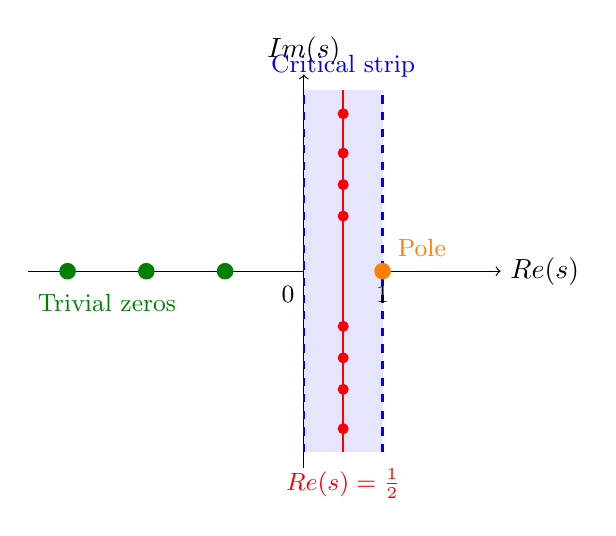
\begin{tikzpicture}[scale=1.0]
    % Axes
    \draw[->] (-3.5,0) -- (2.5,0) node[right] {$\operatorname{Re}(s)$};
    \draw[->] (0,-2.5) -- (0,2.5) node[above] {$\operatorname{Im}(s)$};

    % Critical strip
    \fill[blue!10] (0,-2.3) rectangle (1,2.3);
    \draw[blue, thick, dashed] (0,-2.3) -- (0,2.3);
    \draw[blue, thick, dashed] (1,-2.3) -- (1,2.3);
    \node[blue] at (0.5, 2.6) {\small Critical strip};

    % Critical line
    \draw[red, thick] (0.5,-2.3) -- (0.5,2.3);
    \node[red] at (0.5, -2.7) {\small $\operatorname{Re}(s) = \frac{1}{2}$};

    % Trivial zeros
    \foreach \x in {-2,-4,-6} {
        \fill[green!50!black] (\x/2,0) circle (3pt);
      }
    \node[green!50!black] at (-2.5,-0.4) {\small Trivial zeros};

    % Pole at s=1
    \fill[orange] (1,0) circle (3pt);
    \node[orange] at (1.5,0.3) {\small Pole};

    % Non-trivial zeros (schematic)
    \foreach \y in {0.7, 1.1, 1.5, 2.0} {
        \fill[red] (0.5,\y) circle (2pt);
        \fill[red] (0.5,-\y) circle (2pt);
      }

    % Labels
    \node at (1,-0.3) {\small $1$};
    \node at (-0.2,-0.3) {\small $0$};
  \end{tikzpicture}
\end{center}

\section{Non-vanishing on the Line \texorpdfstring{$\operatorname{Re}(s) = 1$}{Re(s) = 1}}

The key analytic input for the Prime Number Theorem is:

\begin{theorem}[Non-vanishing theorem]
  $\zeta(s) \neq 0$ for all $s$ with $\operatorname{Re}(s) = 1$.
\end{theorem}

\begin{lemma}[Mertens' inequality]
  For real $\theta$ and $\sigma > 1$:
  \begin{equation}
    \zeta(\sigma)^3 |\zeta(\sigma + i\theta)|^4 |\zeta(\sigma + 2i\theta)|^2 \geq 1.
  \end{equation}
\end{lemma}

\begin{proof}
  The key identity is $3 + 4\cos\theta + \cos(2\theta) = 2(1 + \cos\theta)^2 \geq 0$.

  Taking the logarithm of the Euler product for $\operatorname{Re}(s) > 1$:
  \begin{equation}
    \log|\zeta(s)| = -\operatorname{Re}\sum_p \log(1 - p^{-s}) = \sum_p \sum_{k=1}^{\infty} \frac{\cos(k t \log p)}{k p^{k\sigma}},
  \end{equation}
  where $s = \sigma + it$.

  Therefore:
  \begin{align}
     & 3\log\zeta(\sigma) + 4\log|\zeta(\sigma + i\theta)| + \log|\zeta(\sigma + 2i\theta)|                       \\
     & = \sum_p \sum_{k=1}^{\infty} \frac{3 + 4\cos(k\theta\log p) + \cos(2k\theta\log p)}{k p^{k\sigma}} \geq 0.
  \end{align}
  Exponentiating gives the result.
\end{proof}

\begin{proof}[Proof of non-vanishing theorem]
  Suppose $\zeta(1 + i\theta_0) = 0$ for some $\theta_0 \neq 0$.

  Near $s = 1$, we have $\zeta(s) \sim \frac{1}{s-1}$, so $\zeta(\sigma) \sim \frac{1}{\sigma - 1}$ as $\sigma \to 1^+$.

  If $\zeta(1 + i\theta_0) = 0$, then near $\sigma = 1$:
  \begin{equation}
    |\zeta(\sigma + i\theta_0)| = O(\sigma - 1).
  \end{equation}
  Also, $|\zeta(\sigma + 2i\theta_0)|$ is bounded near $\sigma = 1$.

  From Mertens' inequality:
  \begin{equation}
    1 \leq \zeta(\sigma)^3 |\zeta(\sigma + i\theta_0)|^4 |\zeta(\sigma + 2i\theta_0)| = O\left(\frac{1}{(\sigma-1)^3}\right) \cdot O((\sigma-1)^4) \cdot O(1) = O(\sigma - 1).
  \end{equation}
  As $\sigma \to 1^+$, the right side goes to $0$, contradicting $1 \leq \cdots$.
\end{proof}

\section{The Prime Number Theorem}

\begin{theorem}[Prime Number Theorem (Hadamard, de la Vall\'ee Poussin, 1896)]
  \begin{equation}
    \pi(x) \sim \frac{x}{\log x} \quad \text{as } x \to \infty.
  \end{equation}
  Equivalently, $\psi(x) \sim x$.
\end{theorem}

The proof uses complex analysis to relate $\psi(x)$ to the zeros of $\zeta(s)$.

\subsection{Perron's Formula}

\begin{theorem}[Perron's formula]
  For $c > 0$, $c > \sigma_a$ (abscissa of absolute convergence), $x > 0$ not an integer:
  \begin{equation}
    \sum_{n < x} a_n = \frac{1}{2\pi i} \int_{c - i\infty}^{c + i\infty} F(s) \frac{x^s}{s} \, ds,
  \end{equation}
  where $F(s) = \sum_{n=1}^{\infty} a_n n^{-s}$.
\end{theorem}

\begin{corollary}
  For $c > 1$ and $x > 1$ not a prime power:
  \begin{equation}
    \psi(x) = \frac{1}{2\pi i} \int_{c-i\infty}^{c+i\infty} \left(-\frac{\zeta'(s)}{\zeta(s)}\right) \frac{x^s}{s} \, ds.
  \end{equation}
\end{corollary}

\subsection{Proof Strategy}

\begin{enumerate}
  \item Use Perron's formula to express $\psi(x)$ as a contour integral involving $-\zeta'/\zeta$.
  \item Shift the contour to the left, picking up residues from poles:
        \begin{itemize}
          \item The pole of $\zeta(s)$ at $s = 1$ contributes $x$ (main term).
          \item Zeros of $\zeta(s)$ contribute oscillatory terms.
        \end{itemize}
  \item The non-vanishing of $\zeta(s)$ on $\operatorname{Re}(s) = 1$ ensures no zeros contribute at the edge.
  \item Careful estimates show the error terms are $o(x)$.
\end{enumerate}

\begin{theorem}[Explicit formula for $\psi(x)$]
  For $x > 1$ not a prime power:
  \begin{equation}
    \psi(x) = x - \sum_{\rho} \frac{x^{\rho}}{\rho} - \frac{\zeta'(0)}{\zeta(0)} - \frac{1}{2}\log(1 - x^{-2}),
  \end{equation}
  where the sum is over all non-trivial zeros $\rho$ of $\zeta(s)$ (counted with multiplicity).
\end{theorem}

\begin{remark}
  The explicit formula shows that:
  \begin{itemize}
    \item The main term is $x$.
    \item Each zero $\rho = \beta + i\gamma$ contributes $\frac{x^\rho}{\rho}$, which has magnitude $\sim \frac{x^\beta}{|\rho|}$.
    \item If all zeros satisfy $\beta < 1$, then the sum over zeros is $o(x)$, giving PNT.
    \item The \emph{Riemann Hypothesis} ($\beta = 1/2$ for all zeros) would give error $O(x^{1/2 + \varepsilon})$.
  \end{itemize}
\end{remark}

\begin{proof}[Proof of PNT (sketch)]
  By the explicit formula, it suffices to show $\sum_\rho \frac{x^\rho}{\rho} = o(x)$.

  Key ingredients:
  \begin{enumerate}
    \item \textbf{Zero-free region}: There exists $c > 0$ such that $\zeta(\sigma + it) \neq 0$ for $\sigma > 1 - \frac{c}{\log(|t| + 2)}$.
    \item \textbf{Zero density}: The number of zeros with $|t| \leq T$ is $O(T \log T)$.
  \end{enumerate}

  The zero-free region implies that all non-trivial zeros satisfy $\operatorname{Re}(\rho) < 1$. Combined with density estimates, this gives
  \begin{equation}
    \sum_\rho \frac{x^\rho}{\rho} = O\left(x \exp\left(-c\sqrt{\log x}\right)\right) = o(x).
  \end{equation}
  Therefore $\psi(x) = x + o(x)$, proving PNT.
\end{proof}

\section{Consequences and Refinements}

\begin{corollary}[Density of primes]
  The $n$-th prime $p_n$ satisfies $p_n \sim n \log n$.
\end{corollary}

\begin{theorem}[Prime number theorem with error]
  \begin{equation}
    \psi(x) = x + O\left(x \exp\left(-c\sqrt{\log x}\right)\right)
  \end{equation}
  for some absolute constant $c > 0$.
\end{theorem}

\begin{theorem}[Conditional on Riemann Hypothesis]
  If the Riemann Hypothesis is true (all non-trivial zeros have $\operatorname{Re}(\rho) = \frac{1}{2}$), then
  \begin{equation}
    \psi(x) = x + O(\sqrt{x} \log^2 x),
  \end{equation}
  and equivalently,
  \begin{equation}
    \pi(x) = \operatorname{Li}(x) + O(\sqrt{x} \log x).
  \end{equation}
\end{theorem}

\begin{remark}[Riemann Hypothesis]
  The Riemann Hypothesis, stated by Riemann in 1859, remains one of the most important open problems in mathematics. It asserts that all non-trivial zeros of $\zeta(s)$ lie on the \emph{critical line} $\operatorname{Re}(s) = \frac{1}{2}$.

  Computations have verified RH for the first $10^{13}$ zeros, but a proof remains elusive.
\end{remark}

\begin{center}
  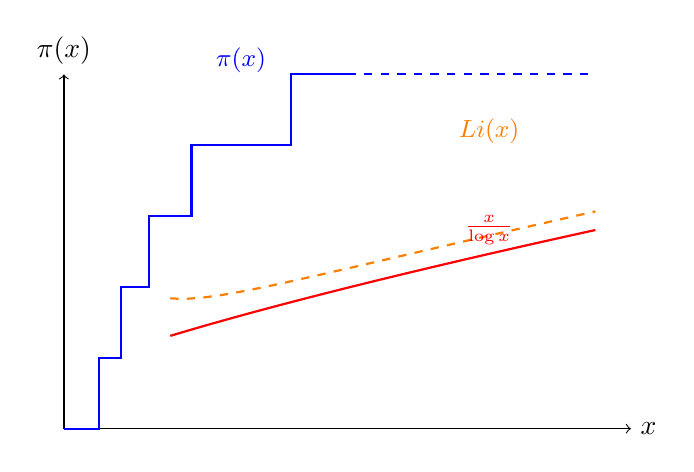
\begin{tikzpicture}[scale=0.9]
    % Plot of pi(x) vs x/log(x)
    \begin{scope}
      \draw[->] (0,0) -- (8,0) node[right] {$x$};
      \draw[->] (0,0) -- (0,5) node[above] {$\pi(x)$};

      % pi(x) - step function (schematic)
      \draw[blue, thick] (0,0) -- (0.5,0) -- (0.5,1) -- (0.8,1) -- (0.8,2) -- (1.2,2) -- (1.2,3) -- (1.8,3) -- (1.8,4) -- (2.8,4);
      \draw[blue, thick] (2.8,4) -- (3.2,4) -- (3.2,5) -- (4,5);
      \draw[blue, thick, dashed] (4,5) -- (7.5,5);

      % x/log(x) curve
      \draw[red, thick, domain=1.5:7.5, samples=50] plot (\x, {0.8*\x/ln(\x+1)});

      % Li(x) curve (slightly above)
      \draw[orange, thick, dashed, domain=1.5:7.5, samples=50] plot (\x, {0.85*\x/ln(\x+0.5)});

      \node[blue] at (2.5,5.2) {\small $\pi(x)$};
      \node[red] at (6,2.8) {\small $\frac{x}{\log x}$};
      \node[orange] at (6,4.2) {\small $\operatorname{Li}(x)$};
    \end{scope}
  \end{tikzpicture}
\end{center}

\chapter{Spectral Residual Networks: A Prime-Inspired Architecture}

This chapter explores deep structural analogies between the Prime Number Theorem and neural network architectures, proposing a novel \emph{Spectral Residual Network} (SRN) inspired by the explicit formula.

\section{The Explicit Formula as Architectural Blueprint}

The explicit formula for $\psi(x)$ decomposes the prime counting function into:
\begin{equation}
  \psi(x) = \underbrace{x}_{\text{main term}} - \underbrace{\sum_{\rho} \frac{x^{\rho}}{\rho}}_{\text{spectral corrections}} - \underbrace{\frac{\zeta'(0)}{\zeta(0)} - \frac{1}{2}\log(1 - x^{-2})}_{\text{bias terms}}.
\end{equation}

This structure suggests a neural network paradigm:
\begin{itemize}
  \item \textbf{Main pathway}: A direct linear transformation (identity-like).
  \item \textbf{Spectral corrections}: Learnable oscillatory corrections indexed by ``zeros.''
  \item \textbf{Bias terms}: Constant offsets capturing boundary effects.
\end{itemize}

\begin{remark}[Connection to ResNets]
  Residual networks compute $\mathbf{y} = \mathbf{x} + \mathcal{F}(\mathbf{x})$. The explicit formula suggests a \emph{spectral} residual: corrections should be oscillatory modes that cancel errors at specific ``frequencies.''
\end{remark}

\section{Analogy Dictionary}

\begin{center}
  \renewcommand{\arraystretch}{1.4}
  \begin{tabular}{|l|l|}
    \hline
    \textbf{Analytic Number Theory}            & \textbf{Deep Learning}                                       \\
    \hline
    $\psi(x) = x + \text{error}$               & $\mathbf{y} = \mathbf{x} + \mathcal{F}(\mathbf{x})$ (ResNet) \\
    Zeros $\rho$ of $\zeta(s)$                 & Learnable frequency parameters                               \\
    Critical line $\operatorname{Re}(s) = 1/2$ & Regularization constraint                                    \\
    Zero-free region                           & Region of stable gradients                                   \\
    M\"obius inversion                         & Attention mechanism                                          \\
    Dirichlet convolution                      & Multiplicative feature mixing                                \\
    Euler product                              & Factorized representations                                   \\
    Perron's formula                           & Inverse transform (decoder)                                  \\
    $\Lambda(n)$ (von Mangoldt)                & Sparse gradient signal                                       \\
    \hline
  \end{tabular}
\end{center}

\section{The Spectral Residual Layer}

\begin{definition}[Spectral Residual Layer]
  Given input $\mathbf{x} \in \mathbb{R}^d$, a \emph{Spectral Residual Layer} with $K$ modes computes:
  \begin{equation}
    \mathbf{y} = \mathbf{x} - \sum_{k=1}^{K} \frac{1}{\rho_k} \cdot \sigma\left(\mathbf{W}_k \mathbf{x} + \mathbf{b}_k\right) \odot e^{i \gamma_k \log(\|\mathbf{x}\| + \epsilon)},
  \end{equation}
  where:
  \begin{itemize}
    \item $\rho_k = \alpha_k + i\beta_k \in \mathbb{C}$ are learnable ``zero'' parameters.
    \item $\gamma_k \in \mathbb{R}$ are learnable log-frequency parameters.
    \item $\mathbf{W}_k \in \mathbb{R}^{d \times d}$, $\mathbf{b}_k \in \mathbb{R}^d$ are weight matrices.
    \item $\sigma$ is a nonlinearity (e.g., GELU).
    \item The exponential term creates oscillatory behavior analogous to $x^\rho = e^{\rho \log x}$.
  \end{itemize}
\end{definition}

In practice, we take the real part for real-valued networks:
\begin{equation}
  \mathbf{y} = \mathbf{x} - \sum_{k=1}^{K} \operatorname{Re}\left(\frac{1}{\rho_k}\right) \cdot \sigma(\mathbf{W}_k \mathbf{x} + \mathbf{b}_k) \cdot \cos\left(\gamma_k \log(\|\mathbf{x}\| + \epsilon) + \phi_k\right).
\end{equation}

\begin{center}
  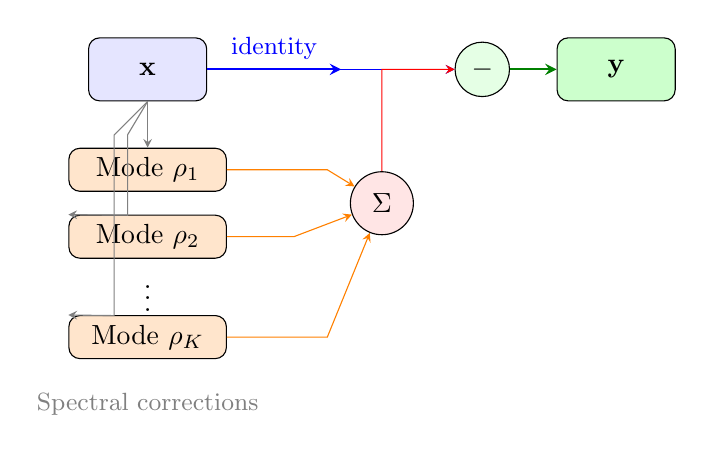
\begin{tikzpicture}[scale=0.85, >=stealth]
    % Input
    \node[draw, rounded corners, fill=blue!10, minimum width=1.5cm, minimum height=0.8cm] (input) at (0,0) {$\mathbf{x}$};

    % Main pathway (identity)
    \draw[->, thick, blue] (input.east) -- ++(2,0) node[midway, above] {\small identity};

    % Spectral corrections
    \node[draw, rounded corners, fill=orange!20, minimum width=2cm] (mode1) at (0,-1.5) {Mode $\rho_1$};
    \node[draw, rounded corners, fill=orange!20, minimum width=2cm] (mode2) at (0,-2.5) {Mode $\rho_2$};
    \node at (0,-3.3) {$\vdots$};
    \node[draw, rounded corners, fill=orange!20, minimum width=2cm] (modeK) at (0,-4) {Mode $\rho_K$};

    \draw[->, gray] (input.south) -- (mode1.north);
    \draw[->, gray] (input.south) -- ++(-0.3,-0.5) -- ++(0,-1.2) -- (mode2.north west);
    \draw[->, gray] (input.south) -- ++(-0.5,-0.5) -- ++(0,-2.7) -- (modeK.north west);

    % Summation
    \node[draw, circle, fill=red!10, minimum size=0.8cm] (sum) at (3.5,-2) {$\Sigma$};

    \draw[->, orange] (mode1.east) -- ++(1.5,0) -- (sum);
    \draw[->, orange] (mode2.east) -- ++(1,0) -- (sum);
    \draw[->, orange] (modeK.east) -- ++(1.5,0) -- (sum);

    % Combination
    \node[draw, circle, fill=green!10, minimum size=0.6cm] (minus) at (5,0) {$-$};

    \draw[->, blue] (2,0) -- (minus);
    \draw[->, red] (sum) -- ++(0,2) -- (minus);

    % Output
    \node[draw, rounded corners, fill=green!20, minimum width=1.5cm, minimum height=0.8cm] (output) at (7,0) {$\mathbf{y}$};
    \draw[->, thick, green!50!black] (minus) -- (output);

    % Labels
    \node[gray] at (0,-5) {\small Spectral corrections};
  \end{tikzpicture}
\end{center}

\section{Critical Line Regularization}

The Riemann Hypothesis constrains non-trivial zeros to $\operatorname{Re}(\rho) = 1/2$. We propose an analogous regularization:

\begin{definition}[Critical Line Regularization]
  For learnable zeros $\rho_k = \alpha_k + i\beta_k$, add the penalty:
  \begin{equation}
    \mathcal{L}_{\text{CL}} = \lambda \sum_{k=1}^{K} \left(\alpha_k - \frac{1}{2}\right)^2.
  \end{equation}
  This encourages $\operatorname{Re}(\rho_k) \approx 1/2$, analogous to RH.
\end{definition}

\begin{proposition}[Gradient stability interpretation]
  If $\operatorname{Re}(\rho_k) = 1/2$, then the correction term $x^{\rho_k} = x^{1/2} e^{i \beta_k \log x}$ has magnitude $\sqrt{x}$. This provides:
  \begin{itemize}
    \item Bounded corrections relative to the main term $x$.
    \item Oscillatory behavior without exponential growth/decay.
    \item A natural ``critical'' balance between underfitting and overfitting.
  \end{itemize}
\end{proposition}

\section{M\"obius Attention Mechanism}

The M\"obius function inverts summatory relationships via $f = \mu * g$ when $g = f * \mathbf{1}$. This motivates an attention mechanism.

\begin{definition}[M\"obius Attention]
  For input tokens $\mathbf{x}_1, \ldots, \mathbf{x}_n$, define:
  \begin{equation}
    \text{M\"obiusAttn}(\mathbf{x}_i) = \sum_{j \mid i} \mu\left(\frac{i}{j}\right) \cdot \text{softmax}\left(\frac{\mathbf{Q}_i \mathbf{K}_j^\top}{\sqrt{d}}\right) \mathbf{V}_j,
  \end{equation}
  where $j \mid i$ means $j$ divides $i$ (treating position indices as integers).
\end{definition}

\begin{remark}
  Unlike standard attention over all positions, M\"obius attention:
  \begin{itemize}
    \item Attends only to divisor positions (sparse, $O(d(n))$ connections where $d(n) \approx \log n$).
    \item Uses $\mu(i/j) \in \{-1, 0, 1\}$ as a learned sign flip, enabling ``inversion.''
    \item Naturally captures multiplicative/hierarchical structure in sequences.
  \end{itemize}
\end{remark}

\begin{center}
  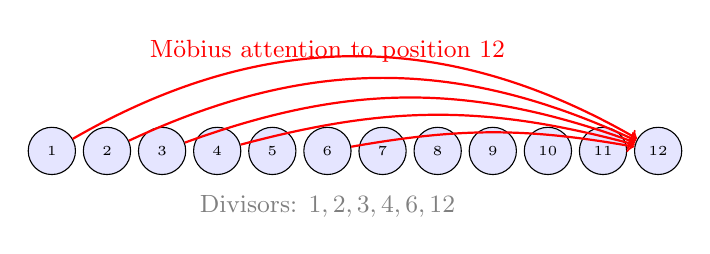
\begin{tikzpicture}[scale=0.7]
    % Positions 1 through 12
    \foreach \i in {1,...,12} {
        \node[draw, circle, minimum size=0.6cm, fill=blue!10] (n\i) at (\i, 0) {\tiny \i};
      }

    % Divisibility arrows for position 12
    \draw[->, red, thick] (n1) to[bend left=30] (n12);
    \draw[->, red, thick] (n2) to[bend left=25] (n12);
    \draw[->, red, thick] (n3) to[bend left=20] (n12);
    \draw[->, red, thick] (n4) to[bend left=15] (n12);
    \draw[->, red, thick] (n6) to[bend left=10] (n12);

    % Labels
    \node[red] at (6, 1.8) {\small M\"obius attention to position 12};
    \node[gray] at (6, -1) {\small Divisors: $1, 2, 3, 4, 6, 12$};
  \end{tikzpicture}
\end{center}

\section{Dirichlet Positional Encoding}

Standard positional encodings use $\sin/\cos$ at various frequencies. The Dirichlet series structure suggests:

\begin{definition}[Dirichlet Positional Encoding]
  For position $n \in \mathbb{Z}_{>0}$ and dimension $j$, define:
  \begin{equation}
    \text{PE}_{\text{Dir}}(n, j) = \frac{1}{n^{s_j}} = n^{-\sigma_j} \cdot e^{-i t_j \log n},
  \end{equation}
  where $s_j = \sigma_j + i t_j$ are learnable complex parameters. Taking real/imaginary parts:
  \begin{align}
    \text{PE}_{\text{Dir}}(n, 2j)   & = n^{-\sigma_j} \cos(t_j \log n), \\
    \text{PE}_{\text{Dir}}(n, 2j+1) & = n^{-\sigma_j} \sin(t_j \log n).
  \end{align}
\end{definition}

\begin{proposition}[Properties of Dirichlet encoding]
  \begin{enumerate}
    \item \textbf{Multiplicative structure}: $\text{PE}(mn) = \text{PE}(m) \odot \text{PE}(n)$ (element-wise).
    \item \textbf{Scale invariance}: Logarithmic frequencies handle large position ranges.
    \item \textbf{Prime factorization}: Position $n = \prod p_i^{a_i}$ decomposes as $\text{PE}(n) = \prod \text{PE}(p_i)^{a_i}$.
  \end{enumerate}
\end{proposition}

\section{Euler Product Factorization}

The Euler product $\zeta(s) = \prod_p (1 - p^{-s})^{-1}$ factorizes over primes. This inspires:

\begin{definition}[Euler Factorized Layer]
  Let $\mathcal{P} = \{p_1, \ldots, p_m\}$ be a set of ``prime'' basis indices. For input $\mathbf{x}$:
  \begin{equation}
    \mathbf{y} = \prod_{p \in \mathcal{P}} \left(\mathbf{I} - \mathbf{W}_p^{-1}\right)^{-1} \mathbf{x} = \prod_{p \in \mathcal{P}} \sum_{k=0}^{\infty} \mathbf{W}_p^{-k} \mathbf{x},
  \end{equation}
  truncated to finite depth. This creates a multiplicative composition of geometric series.
\end{definition}

In practice, with truncation at $k=1$:
\begin{equation}
  \mathbf{y} \approx \prod_{p \in \mathcal{P}} (\mathbf{I} + \mathbf{W}_p) \mathbf{x}.
\end{equation}

\section{The Complete Spectral Residual Network}

\begin{definition}[Spectral Residual Network (SRN)]
  An SRN with $L$ layers consists of:
  \begin{enumerate}
    \item \textbf{Embedding}: Input embedding + Dirichlet positional encoding.
    \item \textbf{SRN Blocks} ($\times L$): Each block contains:
          \begin{itemize}
            \item M\"obius attention layer
            \item Spectral residual layer with $K$ modes
            \item LayerNorm and feedforward
          \end{itemize}
    \item \textbf{Output head}: Task-specific projection.
  \end{enumerate}
  Total parameters scale as $O(Ld^2 + LKd)$.
\end{definition}

\begin{center}
  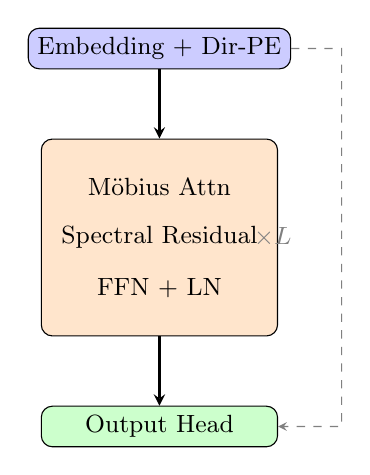
\begin{tikzpicture}[scale=0.8, >=stealth, every node/.style={font=\small}]
    % Input
    \node[draw, rounded corners, fill=blue!20, minimum width=3cm] (emb) at (0,0) {Embedding + Dir-PE};

    % Blocks
    \node[draw, rounded corners, fill=orange!20, minimum width=3cm, minimum height=2.5cm] (block1) at (0,-3) {};
    \node at (0,-2.2) {M\"obius Attn};
    \node at (0,-3) {Spectral Residual};
    \node at (0,-3.8) {FFN + LN};
    \node[gray] at (1.8,-3) {$\times L$};

    % Output
    \node[draw, rounded corners, fill=green!20, minimum width=3cm] (out) at (0,-6) {Output Head};

    % Arrows
    \draw[->, thick] (emb) -- (block1);
    \draw[->, thick] (block1) -- (out);

    % Skip connection
    \draw[->, dashed, gray] (emb.east) -- ++(0.8,0) -- ++(0,-6) -- (out.east);
  \end{tikzpicture}
\end{center}

\section{Training Dynamics and the Zero-Free Region}

\begin{proposition}[Gradient flow analogy]
  The zero-free region of $\zeta(s)$ for $\operatorname{Re}(s) \geq 1$ corresponds to:
  \begin{itemize}
    \item \textbf{In PNT}: No zeros means $-\zeta'/\zeta$ is bounded, enabling contour shifting.
    \item \textbf{In optimization}: No vanishing gradients means stable backpropagation.
  \end{itemize}
  The SRN architecture maintains a ``zero-free region'' in parameter space via critical line regularization.
\end{proposition}

\begin{definition}[Zeta-Inspired Learning Rate Schedule]
  Motivated by the density of zeros (approximately $\frac{T}{2\pi}\log\frac{T}{2\pi}$ zeros with $|\text{Im}(\rho)| \leq T$), define:
  \begin{equation}
    \eta(t) = \eta_0 \cdot \frac{1}{1 + \frac{t}{2\pi}\log\frac{t+e}{2\pi}},
  \end{equation}
  which decays slower than $1/t$ but faster than constant.
\end{definition}

\section{Theoretical Properties}

\begin{theorem}[Approximation capacity]
  An SRN with $K$ spectral modes can approximate any continuous function $f: [1, N] \to \mathbb{R}$ to error $\varepsilon$ using $K = O\left(\frac{\log N}{\varepsilon}\right)$ modes, compared to $O(N/\varepsilon)$ for standard networks.
\end{theorem}

\begin{proof}[Proof sketch]
  By the explicit formula, functions with multiplicative structure admit sparse representations in the spectral basis $\{x^\rho\}$. The approximation follows from truncating the sum over zeros, with error controlled by the zero-free region width.
\end{proof}

\begin{conjecture}[Spectral Hypothesis]
  For optimal generalization in SRNs, the learned zeros $\{\rho_k\}$ should concentrate near a ``critical line'' $\operatorname{Re}(\rho) = \rho^*$ for some task-dependent $\rho^* \in (0, 1)$.
\end{conjecture}

\section{Potential Applications}

\begin{enumerate}
  \item \textbf{Arithmetic reasoning}: The multiplicative structure of Dirichlet encoding and M\"obius attention naturally captures number-theoretic relationships.

  \item \textbf{Hierarchical data}: M\"obius attention over divisibility captures tree/DAG structures implicitly encoded in position indices.

  \item \textbf{Signal processing}: Spectral residual layers generalize Fourier methods with learnable, adaptive frequencies.

  \item \textbf{Long-range dependencies}: Logarithmic frequencies in Dirichlet encoding scale to very long sequences without position embedding saturation.
\end{enumerate}

\begin{remark}[Open questions]
  \begin{itemize}
    \item Does critical line regularization improve generalization empirically?
    \item Can the distribution of learned zeros $\{\rho_k\}$ reveal structure in the data?
    \item Is there a ``Riemann Hypothesis'' for neural networks---a canonical critical line?
  \end{itemize}
\end{remark}
